\section{Payload \& Handler}

\begin{center}
    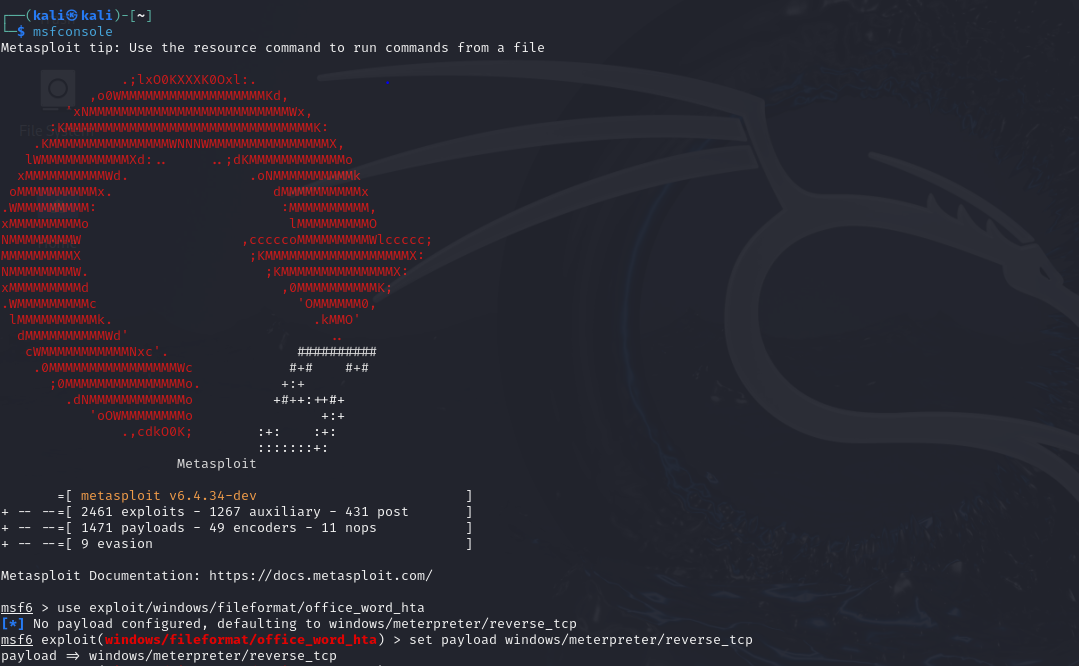
\includegraphics[width=0.8\textwidth]{Question/SC/4_5_6.PNG}
\end{center}

\vspace{0.15cm}

\begin{center}
    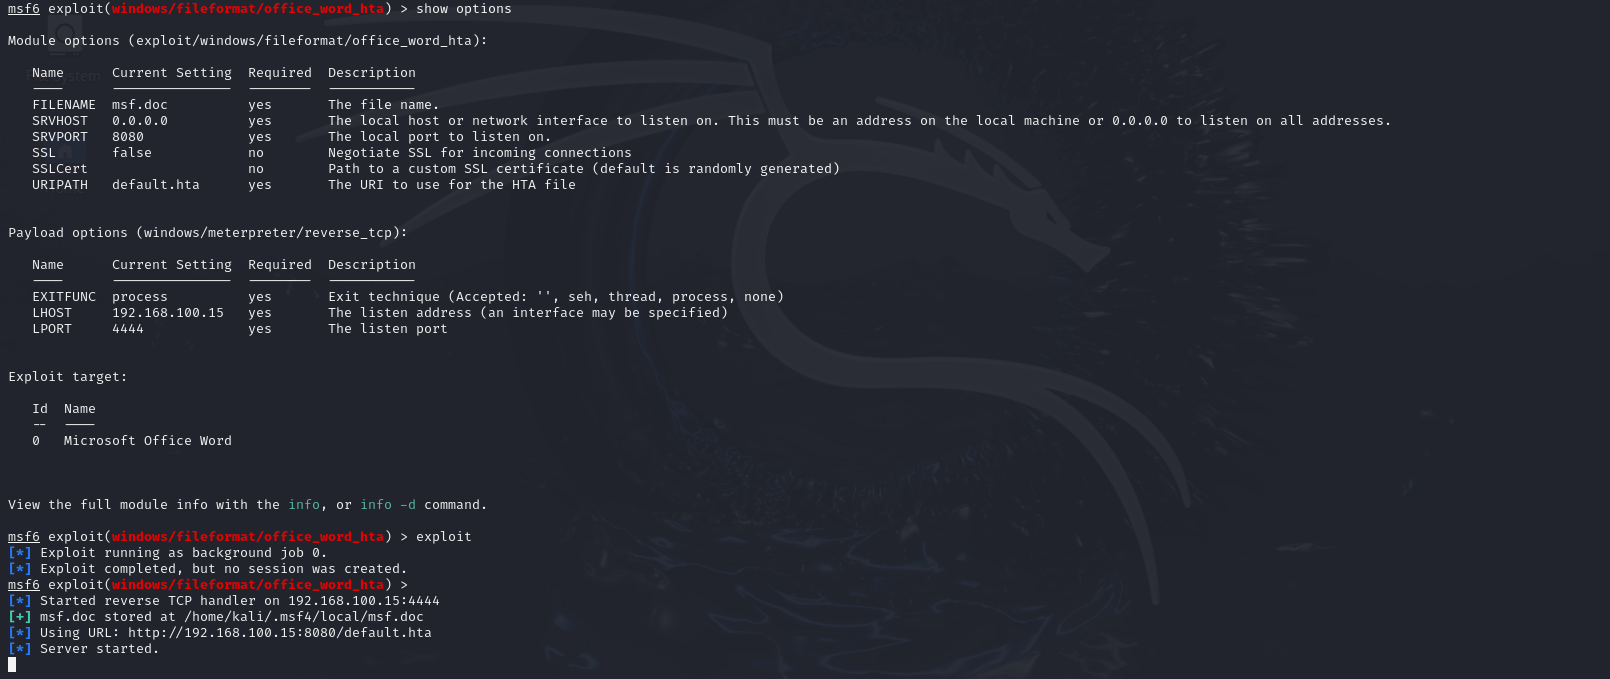
\includegraphics[width=0.8\textwidth]{Question/SC/7_8.PNG}
\end{center}

\vspace{0.35cm}


\begin{prettyBox}{Remarque \& Expliquation}{myblue}
    \begin{itemize}
        \item \textbf{show option} : On remarque que le nom du fichier malveillant est \texttt{msf.doc} 
        \item \textbf{exploit} :
        \begin{itemize}
            \item \textbf{Exploit running as background job 0} :  
        Cela signifie que l'exploit est lancé en tâche de fond (job 0) dans la console Metasploit. Vous pouvez continuer à utiliser la console pendant que ce job s'exécute.
            \item \textbf{Exploit completed, but no session was created} :  
        L'exploit a été exécuté, mais aucune session n'a été établie avec la machine cible. Cela peut indiquer que le payload n'a pas été déclenché ou que la connexion de retour n'a pas été effectuée.
            \item \textbf{Started reverse TCP handler on 192.168.100.15:4444} :  
        Metasploit a démarré un écouteur (handler) en mode reverse TCP à l'adresse IP 192.168.100.15 sur le port 4444. C'est sur ce port que la machine victime devra se connecter pour établir la session Meterpreter.
            \item \textbf{msf.doc stored at /home/kali/.msf4/local/msf.doc} :  
        Le fichier malveillant \texttt{msf.doc} a été généré et sauvegardé dans le répertoire \texttt{/home/kali/.msf4/local/}. Ce fichier est ce qui sera envoyé à la victime pour déclencher le payload.
            \item \textbf{Using URL: https://192.168.100.15:8080/default.hta} :  
        Le module exploite un serveur web interne pour délivrer le payload via une URL. L'URL indiquée montre que le payload (souvent sous forme de script HTA) sera servi depuis l'adresse 192.168.100.15 sur le port 8080.
            \item \textbf{Server Started} :  
        Le serveur HTTP interne de Metasploit est lancé et en attente de connexions. Ce serveur héberge le payload malveillant que la victime devra télécharger et exécuter.        \end{itemize}
    \end{itemize}
\end{prettyBox}

